% questions.tex —— 2004 年·普通高等学校招生考试·浙江卷·文科 · 题目内容片段（无答案）
% 由 tools/generate_projects.py 依来源总账自 2004/2004_数学真题_浙江文科_试题.md 生成，勿手改（改源 MD 后重跑）

\gkpart{一、选择题：本大题共 12 小题，每小题 5 分，共 60 分．在每小题给出的四个选项中，只有一项是符合题目要求的．}

\begin{question}
\gkti{1}若 $U = \{1, 2, 3, 4\}$，$M = \{1, 2\}$，$N = \{2, 3\}$，则 $\complement_U (M \cup N) =$\mbox{（　　）}

\begin{gkopts}(4)
\task A．$\{1, 2, 3\}$
\task B．$\{4\}$
\task C．$\{1, 3, 4\}$
\task D．$\{2\}$
\end{gkopts}

\end{question}
\begin{question}
\gkti{2}直线 $y = 2$ 与直线 $x + y - 2 = 0$ 的夹角是\mbox{（　　）}

\begin{gkopts}(2)
\task A．$\dfrac{\pi}{4}$
\task B．$\dfrac{\pi}{3}$
\task C．$\dfrac{\pi}{2}$
\task D．$\dfrac{3\pi}{4}$
\end{gkopts}

\end{question}
\begin{question}
\gkti{3}已知等差数列 $\{a_n\}$ 的公差为 $2$，若 $a_1, a_3, a_4$ 成等比数列，则 $a_2 =$\mbox{（　　）}

\begin{gkopts}(4)
\task A．$-4$
\task B．$-6$
\task C．$-8$
\task D．$-10$
\end{gkopts}

\end{question}
\begin{question}
\gkti{4}已知向量 $\vec{a} = (3, 4)$，$\vec{b} = (\sin\alpha, \cos\alpha)$，且 $\vec{a} \parallel \vec{b}$，则 $\tan\alpha =$\mbox{（　　）}

\begin{gkopts}(4)
\task A．$\dfrac{3}{4}$
\task B．$-\dfrac{3}{4}$
\task C．$\dfrac{4}{3}$
\task D．$-\dfrac{4}{3}$
\end{gkopts}

\end{question}
\begin{question}
\gkti{5}点 $P$ 从 $(1, 0)$ 出发，沿单位圆 $x^2 + y^2 = 1$ 逆时针方向运动 $\dfrac{2\pi}{3}$ 弧长到达 $Q$ 点，则 $Q$ 的坐标为\mbox{（　　）}

\begin{gkopts}(1)
\task A．$\left(-\dfrac{1}{2}, \dfrac{\sqrt{3}}{2}\right)$
\task B．$\left(-\dfrac{\sqrt{3}}{2}, -\dfrac{1}{2}\right)$
\task C．$\left(-\dfrac{1}{2}, -\dfrac{\sqrt{3}}{2}\right)$
\task D．$\left(-\dfrac{\sqrt{3}}{2}, \dfrac{1}{2}\right)$
\end{gkopts}

\end{question}
\begin{question}
\gkti{6}曲线 $y^2 = 4x$ 关于直线 $x = 2$ 对称的曲线方程是\mbox{（　　）}

\begin{gkopts}(4)
\task A．$y^2 = 8 - 4x$
\task B．$y^2 = 4x - 8$
\task C．$y^2 = 16 - 4x$
\task D．$y^2 = 4x - 16$
\end{gkopts}

\end{question}
\begin{question}
\gkti{7}若 $\left(\sqrt{x} + \dfrac{2}{\sqrt[3]{x}}\right)^n$ 展开式中存在常数项，则 $n$ 的值可以是\mbox{（　　）}

\begin{gkopts}(4)
\task A．$8$
\task B．$9$
\task C．$10$
\task D．$12$
\end{gkopts}

\end{question}
\begin{question}
\gkti{8}在 $\triangle ABC$ 中，“$A > 30^\circ$”是“$\sin A > \dfrac{1}{2}$”的\mbox{（　　）}

\begin{gkopts}(2)
\task A．充分而不必要条件
\task B．必要而不充分条件
\task C．充分必要条件
\task D．既不充分也必要条件
\end{gkopts}

\end{question}
\begin{question}
\gkti{9}若函数 $f(x) = \log_a (x + 1)$（$a > 0, a \neq 1$）的定义域和值域都是 $[0, 1]$，则 $a =$\mbox{（　　）}

\begin{gkopts}(2)
\task A．$\dfrac{1}{3}$
\task B．$\sqrt{2}$
\task C．$\dfrac{\sqrt{2}}{2}$
\task D．$2$
\end{gkopts}

\Needspace{0.4\textheight}
\end{question}
\begin{question}
\gkti{10}如图，在正三棱柱 $ABC - A_1B_1C_1$ 中已知 $AB = 1$，$D$ 在棱 $BB_1$ 上，且 $BD = 1$，若 $AD$ 与平面 $AA_1C_1C$ 所成的角为 $\alpha$，则 $\alpha =$\mbox{（　　）}

\begin{gkopts}(2)
\task A．$\dfrac{\pi}{3}$
\task B．$\dfrac{\pi}{4}$
\task C．$\arcsin\dfrac{\sqrt{10}}{4}$
\task D．$\arcsin\dfrac{\sqrt{6}}{4}$
\end{gkopts}
\nopagebreak[4]
\begin{center}% Candidate source: src-0f11f5c9f471004d5361ba63a8cd76e404c5e126be072fcfb0e205938017cbb2
% Source PDF SHA-256: 2e925ec0caa385c49600a41d3e05877c7c9e7fe13d37904274de8c389e4fd79b
% PDF page 1 (printed page 208), question 10.
% Redraw follows visible/hidden edges: regular triangular prism ABC-A1B1C1, point D on BB1, lines AD and C1A.
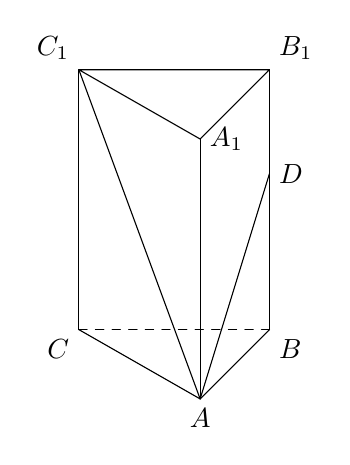
\begin{tikzpicture}[line cap=round,line join=round,>=latex,scale=1.1]
  % Bottom face vertices
  \coordinate (C) at (0,0);
  \coordinate (B) at (2.2,0);
  \coordinate (A) at (1.4,-0.8);

  % Top face vertices (vertical shift 3.0)
  \coordinate (C1) at (0,3.0);
  \coordinate (B1) at (2.2,3.0);
  \coordinate (A1) at (1.4,2.2);

  % Point D on BB1
  \coordinate (D) at (2.2,1.8);

  % Hidden edges
  \draw[dashed] (C) -- (B);

  % Visible edges: bottom face
  \draw (C) -- (A) -- (B);

  % Visible edges: top face
  \draw (C1) -- (A1) -- (B1) -- cycle;

  % Lateral edges
  \draw (C) -- (C1);
  \draw (B) -- (B1);
  \draw (A) -- (A1);

  % Connecting lines AD and C1A
  \draw (A) -- (D);
  \draw (C1) -- (A);

  % Vertex labels
  \node[below left] at (C) {$C$};
  \node[below right] at (B) {$B$};
  \node[below] at (A) {$A$};
  \node[above left] at (C1) {$C_1$};
  \node[above right] at (B1) {$B_1$};
  \node[right] at (A1) {$A_1$};
  \node[right] at (D) {$D$};
\end{tikzpicture}
\end{center}
\nopagebreak[4]
\end{question}
\begin{question}
\gkti{11}若椭圆 $\dfrac{x^2}{a^2} + \dfrac{y^2}{b^2} = 1$（$a > b > 0$）的左、右焦点分别为 $F_1$、$F_2$，线段 $F_1F_2$ 被点 $\left(\dfrac{b}{2}, 0\right)$ 分成 $5 : 3$ 两段，则此椭圆的离心率为\mbox{（　　）}

\begin{gkopts}(2)
\task A．$\dfrac{16}{17}$
\task B．$\dfrac{4\sqrt{17}}{17}$
\task C．$\dfrac{4}{5}$
\task D．$\dfrac{2\sqrt{5}}{5}$
\end{gkopts}

\end{question}
\begin{question}
\gkti{12}若 $f(x)$ 和 $g(x)$ 都是定义在实数集 $\mathbf{R}$ 上的函数，且方程 $x - f[g(x)] = 0$ 有实数解，则 $g[f(x)]$ 不可能是\mbox{（　　）}

\begin{gkopts}(2)
\task A．$x^2 + x - \dfrac{1}{5}$
\task B．$x^2 + x + \dfrac{1}{5}$
\task C．$x^2 - \dfrac{1}{5}$
\task D．$x^2 + \dfrac{1}{5}$
\end{gkopts}

\end{question}
\gkpart{二、填空题：本大题共 4 小题，每小题 4 分，共 16 分．把答案填在题中横线上．}

\begin{question}
\gkti{13}已知 $f(x) = \begin{cases} 1, & x \geqslant 0, \\ -1, & x < 0, \end{cases}$ 则不等式 $x + (x + 2) \cdot f(x + 2) \leqslant 5$ 的解集是 \underline{\hspace{3cm}}．

\end{question}
\begin{question}
\gkti{14}已知平面上三点 $A$、$B$、$C$ 满足 $|\vec{AB}| = 3$，$|\vec{BC}| = 4$，$|\vec{CA}| = 5$，则 $\vec{AB} \cdot \vec{BC} + \vec{BC} \cdot \vec{CA} + \vec{CA} \cdot \vec{AB}$ 的值等于 \underline{\hspace{3cm}}．

\end{question}
\begin{question}
\gkti{15}已知平面 $\alpha \perp \beta$，$\alpha \cap \beta = l$，$P$ 是空间一点，且 $P$ 到 $\alpha$、$\beta$ 的距离分别是 $1$、$2$，则点 $P$ 到 $l$ 的距离为 \underline{\hspace{3cm}}．

\end{question}
\begin{question}
\gkti{16}设坐标平面内有一个质点从原点出发，沿 $x$ 轴跳动，每次向正方向或负方向跳 $1$ 个单位，经过 $5$ 次跳动质点落在点 $(3, 0)$（允许重复过此点）处，则质点不同的运动方法共有 \underline{\hspace{3cm}} 种．（用数字作答）

\end{question}
\gkpart{三、解答题：本大题共 6 小题，共 74 分．解答应写出文字说明、证明过程或演算步骤．}

\begin{question}
\gkti{17}（本小题满分 12 分）

已知数列 $\{a_n\}$ 的前 $n$ 项和为 $S_n$，$S_n = \dfrac{1}{3}(a_n - 1)$（$n \in \mathbf{N}^*$）．

（1）求 $a_1, a_2$；

（2）求证数列 $\{a_n\}$ 是等比数列．

\end{question}
\begin{question}
\gkti{18}（本小题满分 12 分）

在 $\triangle ABC$ 中，角 $A$、$B$、$C$ 所对的边分别为 $a$、$b$、$c$，且 $\cos A = \dfrac{1}{3}$．

（1）求 $\sin^2\dfrac{B+C}{2} + \cos 2A$ 的值；

（2）若 $a = \sqrt{3}$，求 $bc$ 的最大值．

\Needspace{0.4\textheight}
\end{question}
\begin{question}
\gkti{19}（本小题满分 12 分）

如图，已知正方形 $ABCD$ 和矩形 $ACEF$ 所在的平面互相垂直，$AB = \sqrt{2}$，$AF = 1$，$M$ 是线段 $EF$ 的中点．

（1）求证：$AM \parallel$ 平面 $BDE$；

（2）求证：$AM \perp$ 平面 $BDF$；

（3）求二面角 $A - DF - B$ 的大小．
\nopagebreak[4]
\begin{center}% Candidate source: src-0f11f5c9f471004d5361ba63a8cd76e404c5e126be072fcfb0e205938017cbb2
% Source PDF SHA-256: 2e925ec0caa385c49600a41d3e05877c7c9e7fe13d37904274de8c389e4fd79b
% PDF page 1 (printed page 208), question 19.
% Redraw follows visible/hidden edges: square ABCD and rectangle ACEF perpendicular, point M midpoint of EF.
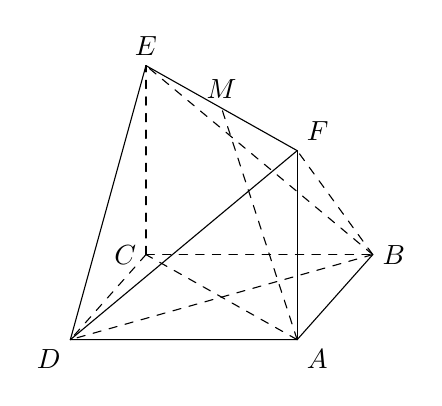
\begin{tikzpicture}[line cap=round,line join=round,>=latex,scale=1.2]
  % Vertex coordinates
  \coordinate (D) at (0,0);
  \coordinate (A) at (2.4,0);
  \coordinate (B) at (3.2,0.9);
  \coordinate (C) at (0.8,0.9);
  \coordinate (F) at (2.4,2.0);
  \coordinate (E) at (0.8,2.9);
  \coordinate (M) at (1.6,2.45);

  % Hidden (dashed) edges
  \draw[dashed] (C) -- (D);
  \draw[dashed] (C) -- (B);
  \draw[dashed] (C) -- (E);
  \draw[dashed] (A) -- (C);
  \draw[dashed] (B) -- (D);
  \draw[dashed] (B) -- (E);
  \draw[dashed] (B) -- (F);
  \draw[dashed] (A) -- (M);

  % Visible (solid) edges
  \draw (D) -- (A) -- (B);
  \draw (A) -- (F);
  \draw (D) -- (E);
  \draw (D) -- (F);
  \draw (E) -- (F);

  % Vertex labels
  \node[below left] at (D) {$D$};
  \node[below right] at (A) {$A$};
  \node[right] at (B) {$B$};
  \node[left] at (C) {$C$};
  \node[above] at (E) {$E$};
  \node[above right] at (F) {$F$};
  \node[above] at (M) {$M$};
\end{tikzpicture}
\end{center}
\nopagebreak[4]
\end{question}
\begin{question}
\gkti{20}（本小题满分 12 分）

某地区有 $5$ 个工厂，由于用电紧缺，规定每个工厂在一周内必须选择某一天停电（选哪一天是等可能的）．假定工厂之间的选择互不影响．

（1）求 $5$ 个工厂均选择星期日停电的概率；

（2）求至少有两个工厂选择同一天停电的概率．

\end{question}
\begin{question}
\gkti{21}（本小题满分 12 分）

已知 $a$ 为实数，$f(x) = (x^2 - 4)(x - a)$．

（1）求导数 $f'(x)$；

（2）若 $f'(-1) = 0$，求 $f(x)$ 在 $[-2, 2]$ 上的最大值和最小值；

（3）若 $f(x)$ 在 $(-\infty, -2]$ 和 $[2, +\infty)$ 上都是递增的，求 $a$ 的取值范围．

\end{question}
\begin{question}
\gkti{22}（本小题满分 14 分）

已知双曲线的中心在原点，右顶点为 $A(1, 0)$，点 $P$、$Q$ 在双曲线的右支上，点 $M(m, 0)$ 到直线 $AP$ 的距离为 $1$．

（1）若直线 $AP$ 的斜率为 $k$，且 $|k| \in \left[\dfrac{\sqrt{3}}{3}, \sqrt{3}\right]$，求实数 $m$ 的取值范围；

（2）当 $m = \sqrt{2} + 1$ 时，$\triangle APQ$ 的内心恰好是点 $M$，求此双曲线的方程．

\end{question}